\section{Introduction}

% In the process of musical composition, composers tend to follow a strict set of theories and guidelines to maintain the aesthetic quality of the music they create \cite{rothgeb1975strict,collins2005synthesis,kikuchi2016music}. The process is usually not standardized and can be customized depending on the task of the composer. As such, one composer's approach might not work effectively for another \cite{cheng2016approaching,collins2016act}. To address this, we present a tool that will assist in the process rather than force composers to adapt to an unnatural approach. We intend to minimize cognitive load in every stage of the composition process. But generally, composers undergo a series of activities that allow them to draft their musical products, regardless of order or sequence \cite{bennett1976process,graf2013beethoven}. These are (1) ideation, (2) sketching, and (3) revision. We developed a product that enables composers to undergo these stages, while ensuring a user-centric approach in the process. \\

Members of the DHH community are unable to fully hear music through conventional means, which may lead to various emotional and social challenges, including expressing emotions \cite{Walker:2013}, making meaningful social connections, and even recognizing their own environment and culture \cite{Ribiero:2017}. One of the solutions developed for this problem is the usage of cochlear implants, which are composed of processors outside of the skin, and an implant placed inside the cochlea. However, cochlear implants do present drawbacks, and may not be sufficient as a stand-alone solution to the problems experienced by the DHH community due to technical limitations \cite{Gfeller:2012, Drennan:2015,Moran:2016}. There have been two main approaches in augmenting the DHH musical experience. The first is through haptic means, to which there have already been several approaches done by previous research \cite{Jack:2015, Nanayakkara:2009:EME, Petry:2016}. The second is through visual means, such as that done by \cite{Jain:2015}, and is the approach taken by this research. This research attempts to make these four (4) contributions: (1) the design of an interaction that seeks to improve how the DHH experience music, (2) the exploration of the use of a movie roll visualization scheme which allows for more creative visuals towards augmenting these experiences \cite{Nanayakkara:2007}, (3) the development of a framework to process and understand music samples towards generating the appropriate visualizations and (4) the evaluation on whether these ultimately augment the music experiences of the DHH.
A framework is introduced following the approach done by \cite{deja2019myosl}, and current work is presented along with the proposed next steps. 

\begin{figure}
     \centering
    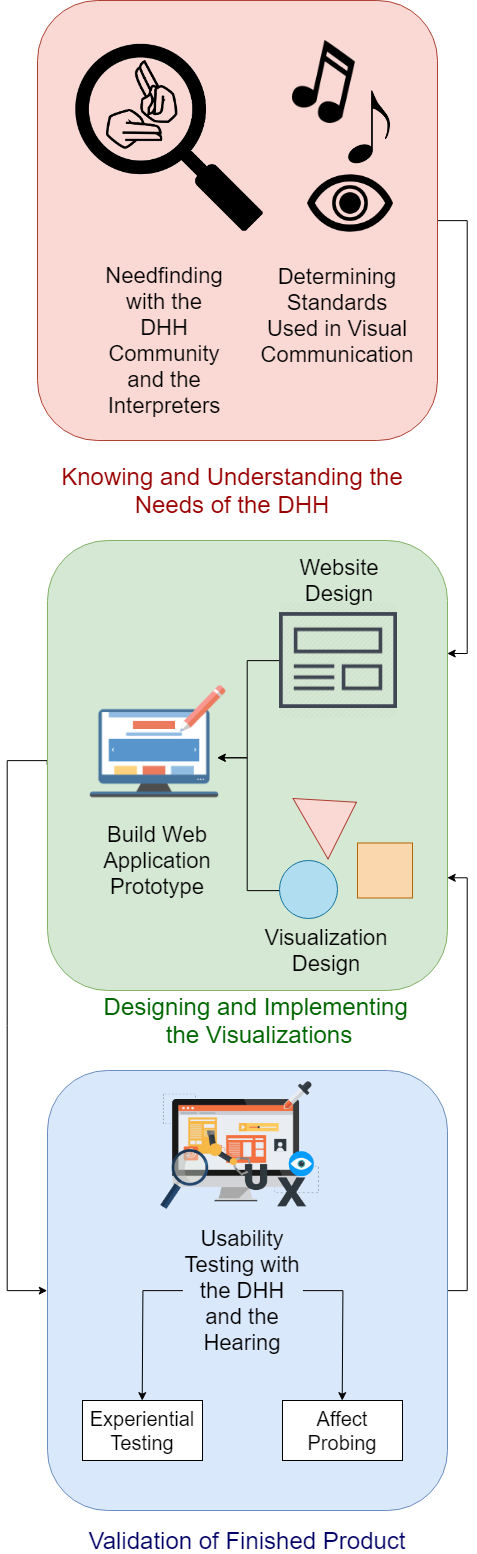
\includegraphics[width=4.5cm,height=12.5cm]{figures/systemDesignFlowchartLite.png}
    \caption{Research Framework}
    \label{fig:research_framework}
\end{figure}

\section{Framework \& Methodology}
    The framework used in this study can be found in Figure \ref{fig:research_framework}.

    
\subsection{Participants}
 The participants were consisted of students and faculty, all of whom are deaf and hard of hearing and 18 to 30 years of age, from the De La Salle-College of Saint Benilde (DLS-CSB) School of Deaf Education and Applied Studies (SDEAS) acquired through coordination with the DLS-CSB SDEAS Office. Two (2) iterations of experiments have been conducted so far, both of which had one (1) interpreter present. Each iteration was conducted with a new set of five (5) participants. This totals to ten (10) respondents who have participated in this study so far. Iteration 1 consisted of four (4) male participants and one (1) female participant. Iteration 2 consisted of three (3) male participants and two (2) female participants.
 
 Each participant signed an informed consent form. Through this, all participants were properly informed of the background of the study, the testing procedures, and how the data acquired from them would be handled. The form states that all data acquired from them linking them to their identities will be kept confidential and will be available to the researchers involved only. Permission to capture their faces and record their feedback and comments was acquired both verbally and through the form. They were made aware that they could withdraw from the experiment at any moment should they wish to do so. 
    
\subsection{Initial Needfinding with the DHH}
Prior to developing the visualization system prototype, needfinding was done with members of the DHH Community. We gathered their thoughts, perspectives, and insights on music, their general experience with it, and how they feel about certain visuals. By getting their point of view, the researchers gained a better understanding of what aspects of music experience is lacking for the deaf, if any. Table \ref{tab:needfinding} shows the list of questions asked to the DHH members. The same questions were asked to interpreters, but in their point of view, based on their knowledge and interactions with the members of the DHH.

\begin{table}
  \centering
  \caption{Initial Needfinding Questions for DHH}~\label{tab:needfinding}
  \addtolength{\tabcolsep}{2pt} 
  \begin{tabular}{p{.5cm}|p{7cm}}
  	\toprule
    \rule{0pt}{8pt}No. & Question \\[2pt]
    \toprule
    Q1 & What are your ideas, definitions, and perspective of music? \\
    Q2 & Which part of the visuals were pleasing to you? Do you experience or feel, physically and emotionally, something when you are exposed to music? If yes, what? \\
    Q3 & Where and when do you usually experience music (ex. concert, mass, car radio, phone)? How do these experiences differ? \\
    Q4 & What methods do you use to experience music? (such as holding balloons at concerts to feel vibrations, watching signers, etc) \\
	Q5 & When people listen to music, they usually react and go along with it, for example, sing. How do you and other deaf and hard of hearing ``sing along''? \\
	Q6 & When people listen to music, they sometimes feel ``chills'' or ``goosebumps'' or tingles on their skin. Do you and other deaf people also get this sensation? \\
	Q7 & Interpreters sometimes sign music, do they enhance your music experience? What is your perspective on these interpretations? \\
	Q8 & What is the difference between signing regular conversations and signing music? \\
	Q9 & When listening to songs with no lyrics, what is expressed to you? \\
	Q10 & What is your perception of musical features such as pitch (highness/lowness), volume, rhythm? How are these translated to you through signing of interpreters (and other methods you may have mentioned)? \\
	Q11 & What do you think are the limitations/shortcomings of the current way of interpreting music to the deaf? \\
	Q12 & From your standpoint, which sensory medium (e.g. sense of sight, sense of touch) do you think would you? \\
	Q13 & What do you think are ways to improve the current methods of translation, especially for music? \\ 
    \bottomrule
  \end{tabular}
  \addtolength{\tabcolsep}{-2pt} 
\end{table}



\subsection{Study Design}
%Our research approach was designed to be iterative, to allow for continuous development and improvement of the prototype. A single iteration involves building the prototype, testing it with composers, and using the resulting feedback and data to improve the next version of the prototype. In every iteration, we collected interaction data through the prototyping application: CogTool. This provided us with measurable data on KLM-GOMS, and Fitts Law \cite{mackenzie1992fitts} without having to measure them manually \cite{sauro2009estimating,bellamy2011deploying}. In each test, the subject was asked to participate in three (3) test setups. The first setup would make the subject use a bare music sheet for composition. The second setup would ask the subjects to use a different mobile musical composition application. The third will make use of our prototype, Flow. The purpose for these setups was to allow us to test our prototype against existing musical composition approaches. Subjects were asked to perform certain tasks (i.e. adding a note, erasing/deleting a note, etc.) in all the test setups. This helped us see the differences of how the users interacted with the setup for a certain task. For the test setup of Flow, the tasks were also meant to test the features shown in Table \ref{tab:features} for the first iteration and additional features shown in Table \ref{tab:features2} for the second iteration. After finishing the tasks in all test setups, the subjects were asked to answer a questionnaire. The questions can be seen in Table \ref{tab:questions}. Note that each of the questions were repeated for each feature (Shown in \ref{tab:features}). The questionnaire aims to get quantitative data on the subject's experience while using Flow. Answers are on a scale of 1 - 4, with 1 (Never or Strongly Disagree) being the lowest, and 4 (Frequently or Strongly Agree) being the highest. 

Our approach follows an iterative format, to allow for continuous development and improvement of the prototype by soliciting user feedback on all phases of development. A total of two (2) iterations were done. The first iteration involved creating the initial prototype, with basic visuals that respond to the music being played. Using the resulting feedback and data, the succeeding iterations focused on improving the visualizer prototype, adjusting the visuals to more appropriately represent the musical features, in hopes to gain more insights from the participants in the next tests. Changes were also made in the setup and testing protocol per iteration based on observations and feedback from participants from previous iterations.

Each iteration is done in two major steps: Step 1 involved allowing the respondents to use the prototype which then leads to Step 2 where the team gets to dive deeper into their feedback and insights in the form of a Focus Group Discussion (FGD). For Step 1, participants were made to listen to and watch the visuals of a playlist of twenty-five (25) songs. The songs were chosen in such a way that the playlist had a balanced variety of music with different characteristics. The songs had different speeds and loudness. Sixteen (16) had lyrics or vocals while the remaining nine (9) did not. The faces of the participants were captured we could review their reactions afterward. Feedback forms were also provided for them to note down their feelings and comments on the visuals per song. Each prototype testing lasted for an approximate of 30 minutes. Step 2 involved an FGD, where participants were asked questions on their experience, and they were asked to expound more than on the feedback form. By doing this, we were able to identify what needed more improvement and focus in the prototype and experiment setup for succeeding iterations. Each FGD lasted for an approximate of 30 minutes.

The feedback form for Iteration 1 contained a table wherein the cells were the songs in the playlist. Each cell only had the title of the song and a blank space where the participant could write any form of comment or feedback. A snippet of this form is shown in Figure \ref{fig:iter1feedback}, while the Iteration 1 FGD questions list can be found in Table \ref{tab:QI1}.

\begin{figure}[h]
	\centering
	\includegraphics[width=0.75\columnwidth]{figures/emotionFaces.png}
    \caption{Snippet of the feedback form used in Iteration 1}
    \label{fig:iter1feedback}
\end{figure}

\begin{table}
  \centering
  \caption{Iteration 1 FGD Questions}~\label{tab:QI1}
  \addtolength{\tabcolsep}{2pt} 
  \begin{tabular}{p{.5cm}|p{7cm}}
  	\toprule
    \rule{0pt}{8pt}No. & Question \\[2pt]
    \toprule
    Q1 & At any point, did the visuals make you feel (Excited / Happy / Relaxed / Contented / Bored / Sad / Tense / Upset)? Why/what caused it? What song did make you feel this way, if you could remember it? \\
    Q2 & Which part of the visuals were pleasing to you? \\
    Q3 & Which part of the visuals were not pleasing to you? \\
    Q4 & Did the visuals help you appreciate the music better? How? \\
	Q5 & How could we improve your experience of music through these visualizations? What visual elements should we add to make your experience better? \\
	Q6 & How else could we improve your experience of music in general? \\
	Q7 & Are there any more comments you would like to add? \\
    \bottomrule
  \end{tabular}
  \addtolength{\tabcolsep}{-2pt} 
\end{table}

After feedback was acquired from Iteration 1, some changes to the experiment setup was made in Iteration 2 based on the suggestions and comments from the participants. Rather than providing each participant with their own device with the prototype and earphones so that they may use at their own pace, the participants all watched the visuals together on a single screen. A large speaker was also pointed downward at the table where their hands were placed to provide vibrational feedback and sound. All participants from Iteration 1 agreed to the suggestion of this setup as they said it would be more enjoyable to them. The feedback form was also revised. It contained a table having one row per song with checkboxes for each affect. The participants were allowed to check the box of each affect that applied. A snippet of this feedback form is shown in \ref{fig:iter2feedback}. The updated list of FGD questions for Iteration 2 can be found in Table \ref{tab:QI2}.

\begin{figure}[h]
	\centering
	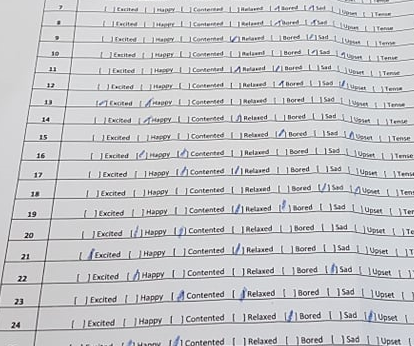
\includegraphics[width=1\columnwidth]{figures/checkboxes.png}
    \caption{Sample Iteration 2 Feedback Form}
    \label{fig:iter2feedback}
\end{figure}

\begin{table}
  \centering
  \caption{Iteration 2 FGD Questions}~\label{tab:QI2}
  \addtolength{\tabcolsep}{2pt} 
  \begin{tabular}{p{.5cm}|p{7cm}}
  	\toprule
    \rule{0pt}{8pt}No. & Question \\[2pt]
    \toprule
    Q1 & What were the feelings you had while watching the visualizations? What visuals made you feel this way? \\
    Q2 & What do you think of the shapes used? Are there others you want to see? \\
    Q3 & What do you think of the colors used? Were they appropriate? \\
    Q4 & Which part of the visuals were pleasing to you? \\
	Q5 & Which part of the visuals were not pleasing to you? \\
	Q6 & Did the visuals help you appreciate the music better? How? \\
	Q7 & How could we improve your experience of music through these visualizations? What visual elements should we add to make your experience better? \\
	Q8 & How else could we improve your experience of music in general? \\
	Q9 & Are there any more comments you would like to add? \\
    \bottomrule
  \end{tabular}
  \addtolength{\tabcolsep}{-2pt} 
\end{table}

%NOTE: Not sure pa, depends ano mangyari sa 3rd iteration
%Iteration 3 was more different from the first two iterations. Each participant had their own separate and individual testing session so as to be more intimate and personal. They were made to listen to and watch the visuals of songs in a playlist, and their faces were still recorded with their consent. Rather than having them note their feelings and comments while watching and expound on them in a Focus Group Discussion afterwards, they were made to view their own recording, and note their feelings and comments at certain timestamps. This protocol allowed for them to be more focused on the experience while watching, and more detailed with their feedback on the form afterwards.

%Insert 3rd iteration sample form

\subsection{Data \& Analysis}
% To add
The data acquired from the experiments were both quantitative and qualitative. Although the data obtained from the feedback forms were qualitative, we were able to convert them into quantitative form. The data from each FGD were purely qualitative. The comments and suggestions made by the participants in the FGD were taken into consideration when changes were made in improving the system prototype.

The data acquired in the feedback forms for Iteration 1 were in the forms of emoticons and words describing the feelings of the participants, such as what is shown in Figure \ref{fig:iter1feedback}. These were mapped to a likert scale of numeric values ranging from 1 to 5. The resulting numeric values were treated as the participant's scores per song. Statistical analysis was then performed by computing the average score and standard deviation per song. Both were used to calculate their correlational coefficients with the BPM of the songs.

The data acquired in the feedback forms for Iteration 2 were in the form of checkmarks, as shown in Figure \ref{fig:iter2feedback}. The number of checkmarks per affect per song were tallied into a table. The resulting quantitative data were then treated statistically by computing the correlational coefficient between the BPM of the song and each affect.

\section{Prototype Features}
The prototype was designed as a web application to allow for more accessibility. It was built using HTML, Javascript, and Nodejs. The p5.js library was used for processing the sound files. It has several useful pre-defined functions, such as performing Fast Fourier Transform (FFT) and beat detection. The Iteration 1 prototype was focused more on getting the visuals to respond to the music in a more or less appropriate manner. The frequency spectrum is acquired at every time frame through FFT. It is then divided evenly into four (4). The first quarter is used for the background. The second quarter is used for the lowground, represented as two (2) large circles. The third quarter is used for the highground, represented as three (3) medium circles. The last quarter is used for the foreground, represented as seven (7) smaller circles. The amplitude at each frequency determines the colors and sizes of these visual elements. For this iteration, grayscale color scheme was used. A diagram of the initial prototype structure is shown in Figure \ref{fig:iter1Struct}. A sample of the visuals produced by the prototype can be seen in Figure  \ref{fig:visuals}(A).

\begin{figure*}[h]
	\centering
	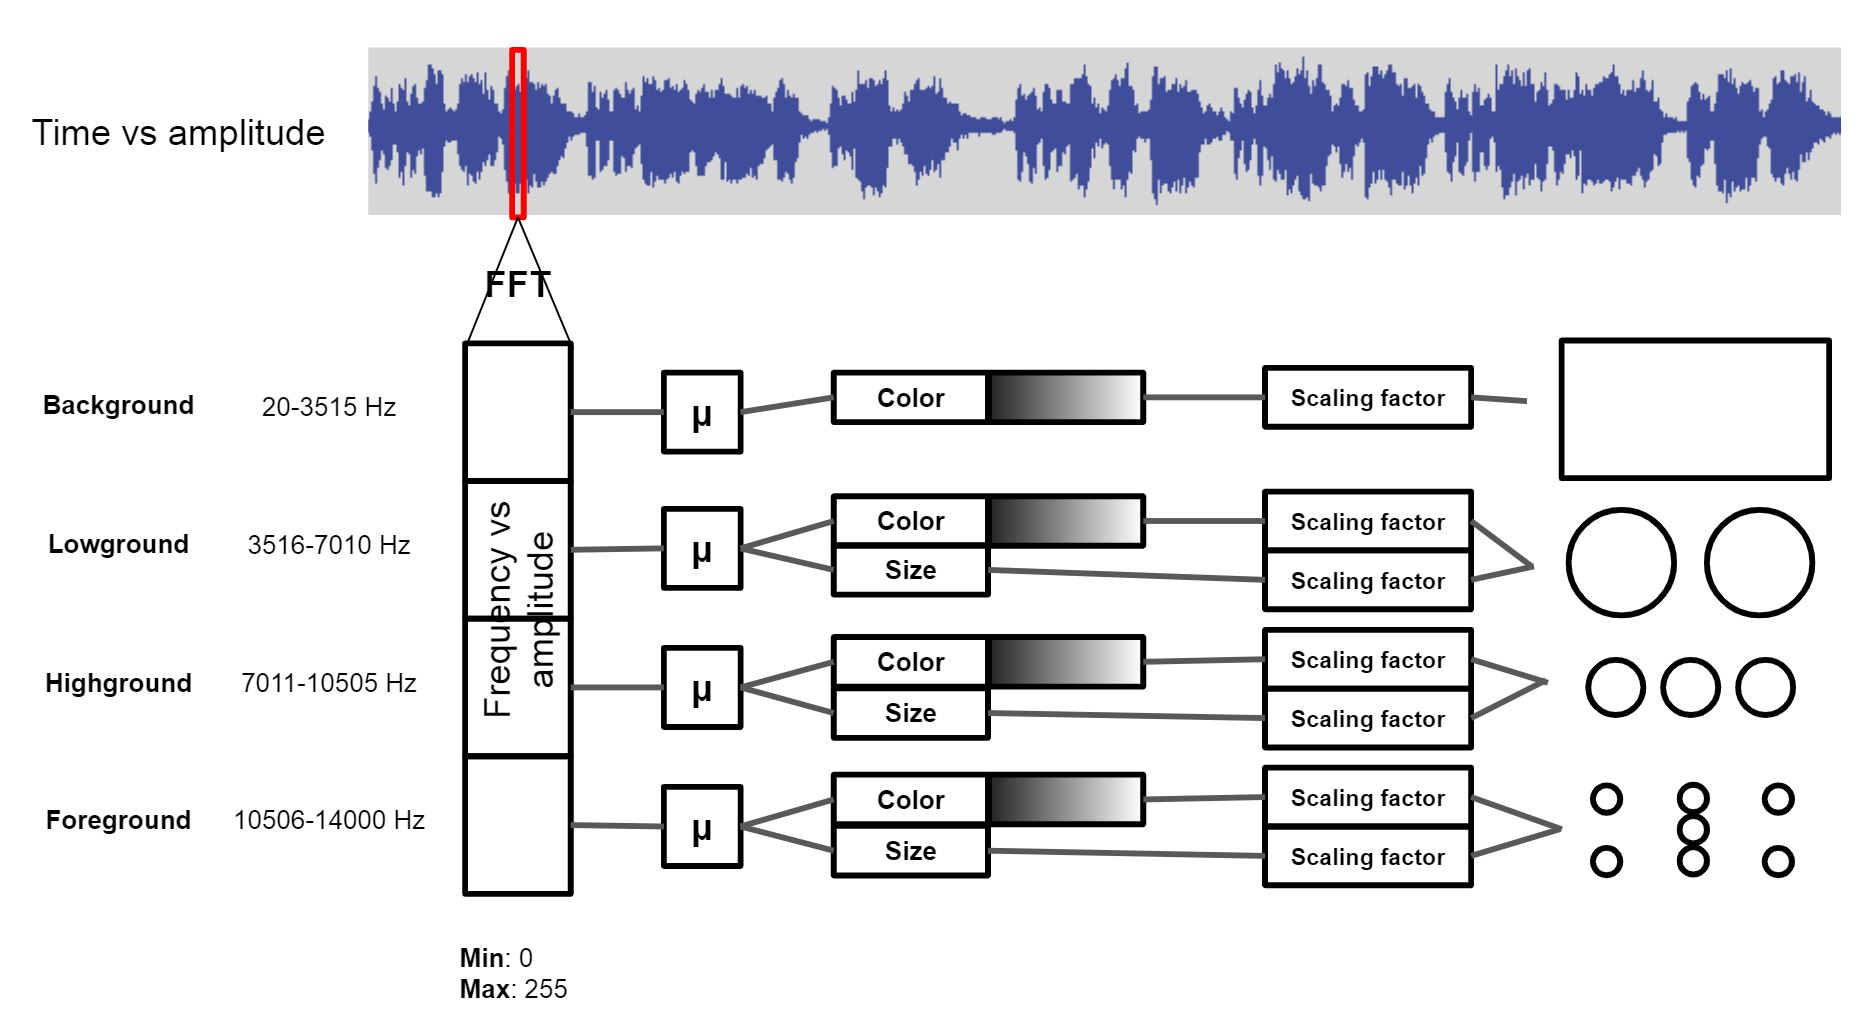
\includegraphics[width=2\columnwidth]{figures/iter1Struct.JPG}
    \caption{Diagram describing the architectural framework of Iteration 1 Prototype}
    \label{fig:iter1Struct}
\end{figure*}

% Iteration 2 explanation
Based on feedback gained from the Iteration 1 prototype testing, some of the visuals were changed for the Iteration 2 prototype. Rather than dividing the frequency spectrum equally, it was divided based on some related literature. A pitch detector component was added and each division in the spectrum runs through it, determining the color of the associated visual elements. Instead of having seven (7) circles to represent the foreground, there are nine (9) star shapes. Particle effects were also added. The particle effects are triggered during increases of amplitude over a period of time. A diagram of the initial prototype structure is shown in Figure \ref{fig:iter2Struct}. A sample of the visuals produced by the prototype can be seen in Figure  \ref{fig:visuals}(B).

\begin{figure*}[h]
	\centering
	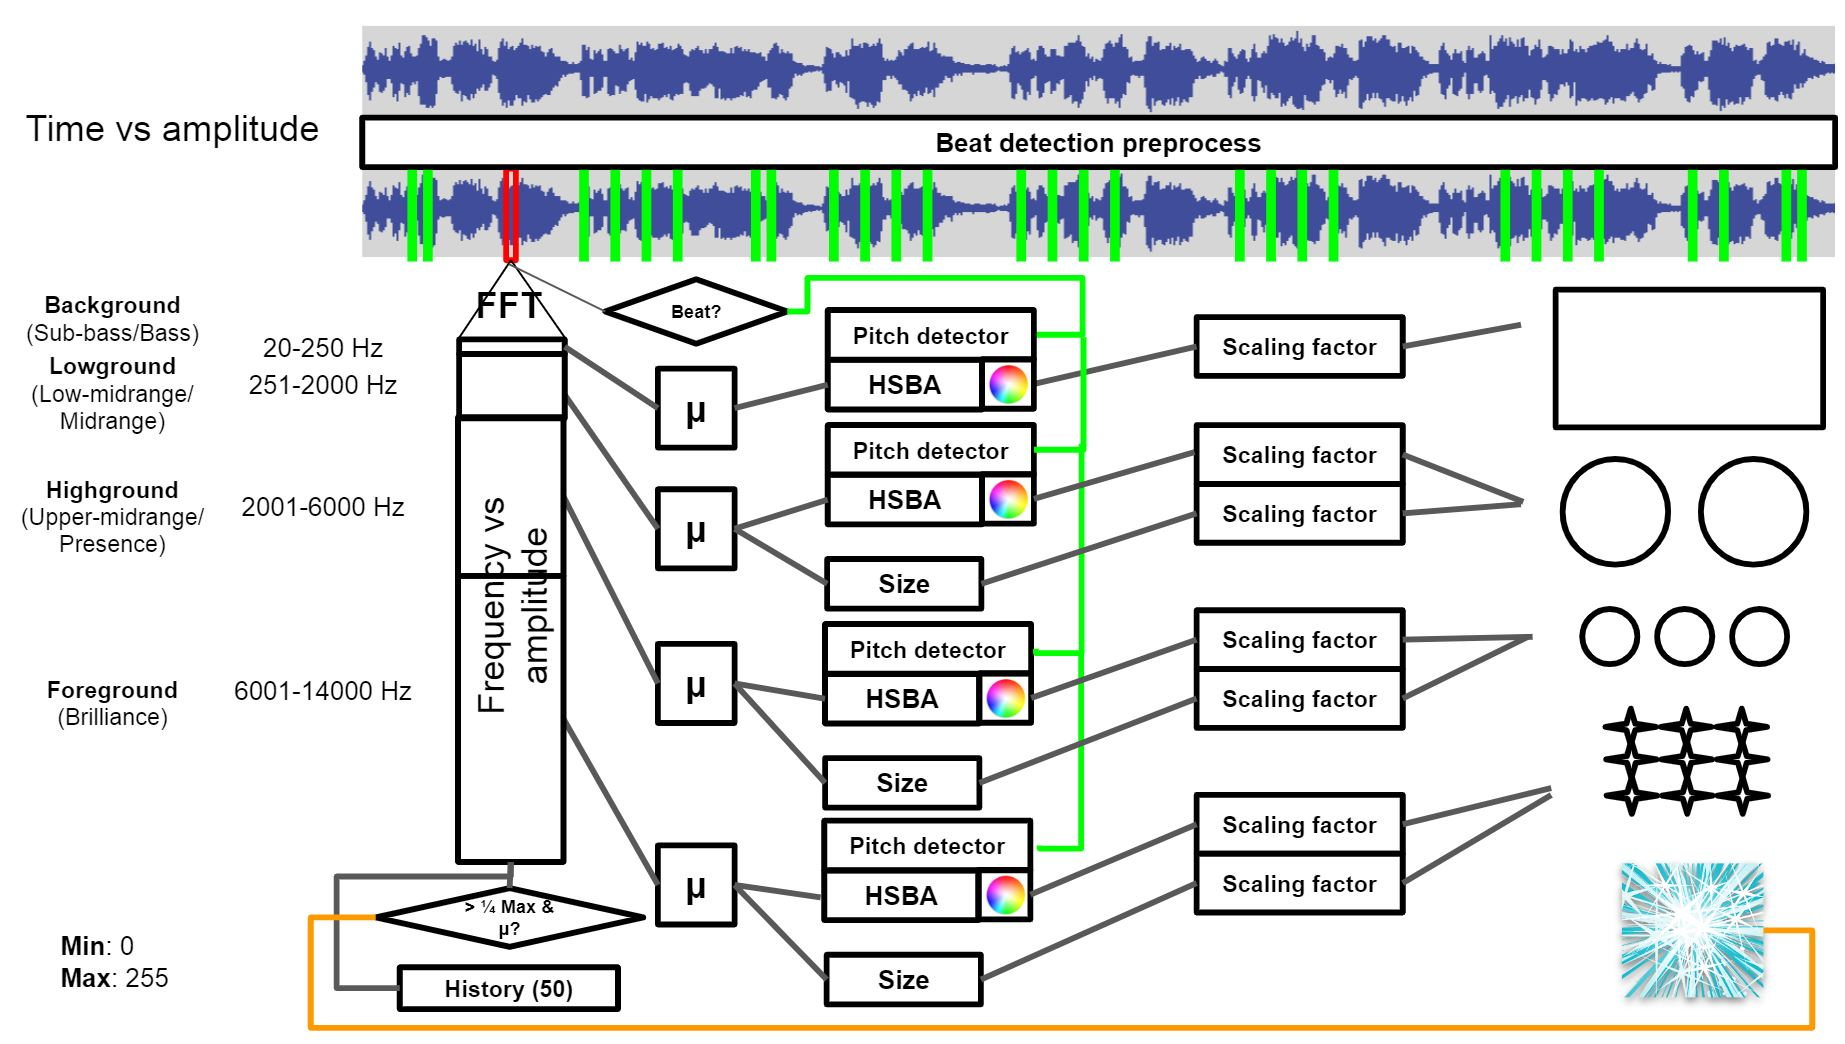
\includegraphics[width=2\columnwidth]{figures/iter2Struct.JPG}
    \caption{Diagram describing the architectural framework of Iteration 2 Prototype}
    \label{fig:iter2Struct}
\end{figure*} 

\begin{figure*}[h]
	\centering
	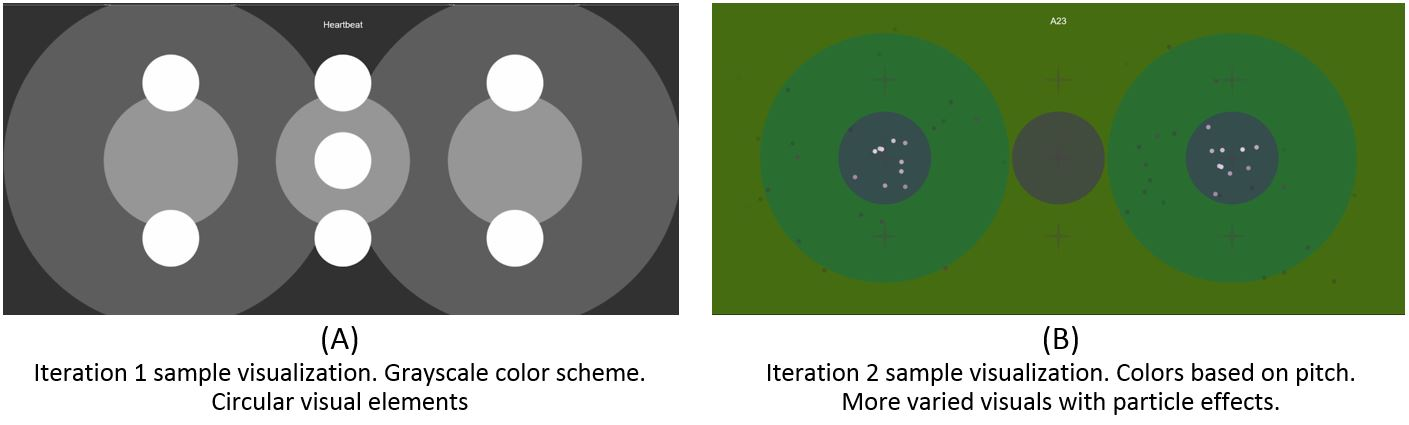
\includegraphics[width=2\columnwidth]{figures/visuals.JPG}
    \caption{Iterations 1 and 2 Prototype Sample Visuals}
    \label{fig:visuals}
\end{figure*} 

% Iteration 3 explanation

\section{Results}

\subsection{Testing Results}

Table \ref{tab:iter1results} shows the overview of the results from the acquired data from the feedback form from Iteration 1, while Table \ref{tab:iter2results} shows the results from Iteration 2. As mentioned, the feedback forms from those iterations differed, so the results and treatment of the data will be discussed separately in the following subsections.

\subsection{Iteration 1} 

% \begin{figure}[H]
% 	\centering
% 	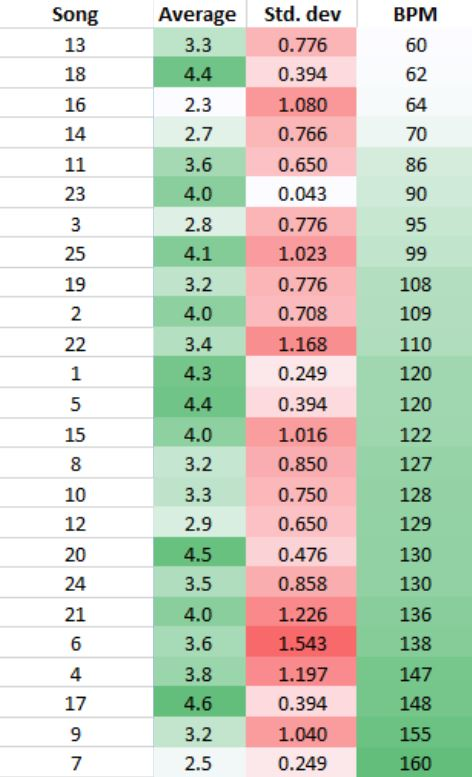
\includegraphics[width=0.8\columnwidth]{figures/iter1results.JPG}
%     \caption{Iteration 1 Feedback Form Results}
%     \label{fig:iter1results}
% \end{figure} 

\begin{table}
  \centering
  \caption{Iteration 1 Feedback Form Results}~\label{tab:iter1results}
  \addtolength{\tabcolsep}{2pt} 
  \begin{tabular}{P{1cm}|P{1.5cm}|P{2cm}|P{1.5cm}}
  	\toprule
    \rule{0pt}{8pt}Song & Average & Std. Dev. & BPM \\[2pt]
    \toprule
    13 & 3.3 & 0.776 & 60 \\ \hline
    18 & 4.4 & 0.394 & 62 \\ \hline
    16 & 2.3 & 1.080 & 64 \\ \hline
    14 & 2.7 & 0.766 & 70 \\ \hline
    11 & 3.6 & 0.650 & 86 \\ \hline
    23 & 4.0 & 0.043 & 90 \\ \hline
    3 & 2.8 & 0.776 & 95 \\ \hline
    25 & 4.1 & 1.023 & 99 \\ \hline
    19 & 3.2 & 0.776 & 108 \\ \hline
    2 & 4.0 & 0.708 & 109 \\ \hline
    22 & 3.4 & 1.168 & 110 \\ \hline
    1 & 4.3 & 0.249 & 120 \\ \hline
    5 & 4.4 & 0.394 & 120 \\ \hline
    15 & 4.0 & 1.016 & 122 \\ \hline
    8 & 3.2 & 0.850 & 127 \\ \hline
    10 & 3.3 & 0.750 & 128 \\ \hline
    12 & 2.9 & 0.650 & 129 \\ \hline
    20 & 4.5 & 0.476 & 130 \\ \hline
    24 & 3.5 & 0.858 & 130 \\ \hline
    21 & 4.0 & 1.226 & 136 \\ \hline
    6 & 3.6 & 1.543 & 138 \\ \hline
    4 & 3.8 & 1.197 & 147 \\ \hline
    17 & 4.6 & 0.394 & 148 \\ \hline
    9 & 3.2 & 1.040 & 155 \\ \hline
    7 & 2.5 & 0.249 & 160 \\
    \bottomrule
  \end{tabular}
  \addtolength{\tabcolsep}{-2pt} 
\end{table}

Based on observations and comments from the Focus Group Discussions, participants appreciated and had a more positive response to the louder and faster songs. All participants agreed that the inclusion of speakers for haptic feedback and colors would improve their experience, as such this was considered for the Iteration 2 experiments. The participants were easily bored due to the grayscale color scheme of the prototype. The participants provided more recommendations such as (1) adding the lyrics as captions (2) visuals of the singer singing the song and (3) adding more visual elements.

Based on the data in Figure \ref{tab:iter1results}, we computed for the correlation coefficients of BPM with average score and BPM with standard deviation, which can be seen in Table \ref{tab:correlations}. Based on these statistical figures, BPM and average score, as well as standard deviation have no correlation.
%The computed correlation coefficient for BPM and average score is 0.1294, which is interpreted as little positive correlation. The computed correlation coefficient for BPM and standard deviation is 0.1145, which is also interpreted as little correlation.

Despite the explicit statements from the participants that they appreciated the louder and faster songs, analysis of the statistical results show that their scores were not consistent. Faster and louder songs did not necessarily have the higher ratings. This may be attributed to mismatches regarding visual impact. The songs may not have had their musical features represented consistently and fairly enough for them to appreciate the experience.

\begin{table}
  \centering
  \caption{Iteration 1 and 2 Computed Correlational Figures}~\label{tab:correlations}
  \addtolength{\tabcolsep}{2pt} 
  \begin{tabular}{P{2.5cm}|P{2.5cm}|P{1.5cm}}
  	\toprule
    \rule{0pt}{8pt}Iteration 1 &  & BPM \\[2pt]
    \toprule
     & Average Score & 0.1294 \\ \hline
     & Std. Dev. & 0.1145 \\
    \bottomrule
    \toprule
    \rule{0pt}{8pt}Iteration 2 &  & BPM \\[2pt]
    \toprule
     & Excitement & 0.0098 \\ \hline
     & Happiness & 0.4397 \\ \hline
     & Contentment & 0.2918 \\ \hline
     & Relaxment & -0.2126 \\ \hline
     & Boredom & -0.183 \\ \hline
     & Sadness & -0.1509 \\ \hline
     & Upsetness & -0.3310 \\ \hline
     & Tension & -0.1500 \\
    \bottomrule
  \end{tabular}
  \addtolength{\tabcolsep}{-2pt} 
\end{table}

\subsection{Iteration 2}

% \begin{figure}[H]
% 	\centering
% 	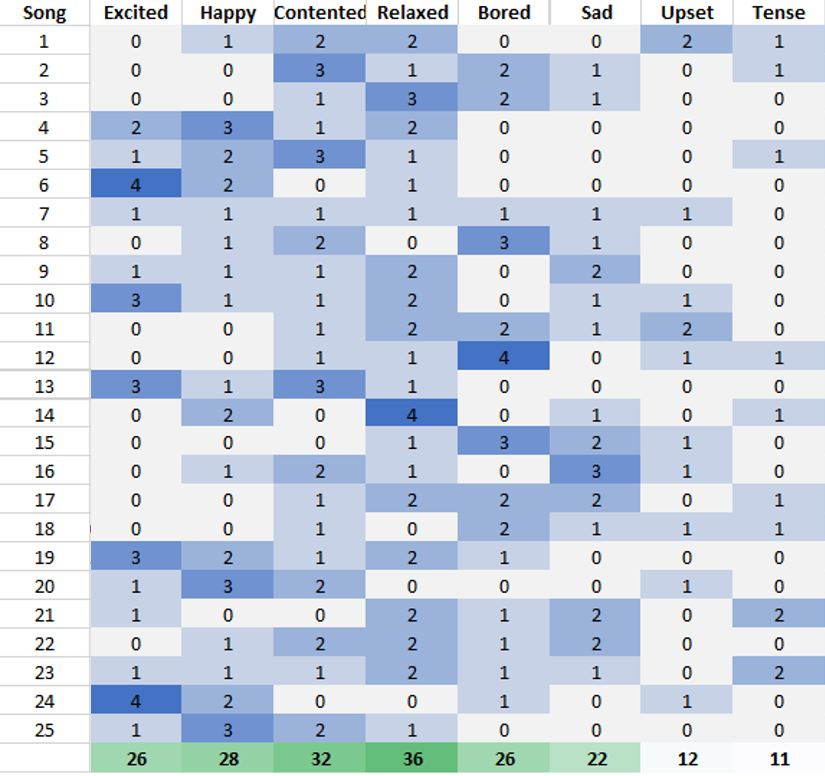
\includegraphics[width=1\columnwidth]{figures/iter2results.JPG}
%     \caption{Iteration 2 Feedback Form Results}
%     \label{fig:iter2results}
% \end{figure}

\begin{table*}[t]
  \centering
  \caption{Iteration 2 Feedback Form Results}~\label{tab:iter2results}
  \addtolength{\tabcolsep}{2pt} 
  \begin{tabular}{P{2.5cm}|P{1cm}|P{0.9cm}|P{1cm}|P{1cm}|P{0.9cm}|P{0.9cm}|P{0.9cm}|P{0.9cm}|>{\bfseries}P{2.5cm}}
  	\toprule
    \rule{0pt}{8pt}Song & Excited & Happy & Content & Relaxed & Bored & Sad & Upset & Tense & Total per Song\\[2pt]
    \toprule
    1 & 0 & 1 & 2 & 2 & 0 & 0 & 2 & 1 & 8 \\ \hline
    2 & 0 & 0 & 3 & 1 & 2 & 1 & 0 & 1 & 8 \\ \hline
    3 & 0 & 0 & 1 & 3 & 2 & 1 & 0 & 0 & 7 \\ \hline
    4 & 2 & 3 & 1 & 2 & 0 & 0 & 0 & 0 & 8 \\ \hline
    5 & 1 & 2 & 3 & 1 & 0 & 0 & 0 & 1 & 8 \\ \hline
    6 & 4 & 2 & 0 & 1 & 0 & 0 & 0 & 0 & 7 \\ \hline
    7 & 1 & 1 & 1 & 1 & 1 & 1 & 1 & 0 & 7 \\ \hline
    8 & 0 & 1 & 2 & 0 & 3 & 1 & 0 & 0 & 7 \\ \hline
    9 & 1 & 1 & 1 & 2 & 0 & 2 & 0 & 0 & 7 \\ \hline
    10 & 3 & 1 & 1 & 2 & 0 & 1 & 1 & 0 & 9 \\ \hline
    11 & 0 & 0 & 1 & 2 & 2 & 1 & 2 & 0 & 8 \\ \hline
    12 & 0 & 0 & 1 & 1 & 4 & 0 & 1 & 1 & 8 \\ \hline
    13 & 3 & 1 & 3 & 1 & 0 & 0 & 0 & 0 & 8 \\ \hline
    14 & 0 & 2 & 0 & 4 & 0 & 1 & 0 & 1 & 8 \\ \hline
    15 & 0 & 0 & 0 & 1 & 3 & 2 & 1 & 0 & 7 \\ \hline
    16 & 0 & 1 & 2 & 1 & 0 & 3 & 1 & 0 & 8 \\ \hline
    17 & 0 & 0 & 1 & 2 & 2 & 2 & 0 & 1 & 8 \\ \hline
    18 & 0 & 0 & 1 & 0 & 2 & 1 & 1 & 1 & 6 \\ \hline
    19 & 3 & 2 & 1 & 2 & 1 & 0 & 0 & 0 & 9 \\ \hline
    20 & 1 & 3 & 2 & 0 & 0 & 0 & 1 & 0 & 7 \\ \hline
    21 & 1 & 0 & 0 & 2 & 1 & 2 & 0 & 2 & 8 \\ \hline
    22 & 0 & 1 & 2 & 2 & 1 & 2 & 0 & 0 & 8 \\ \hline
    23 & 1 & 1 & 1 & 2 & 1 & 1 & 0 & 2 & 9 \\ \hline
    24 & 4 & 2 & 0 & 0 & 1 & 0 & 1 & 0 & 8 \\ \hline
    25 & 1 & 3 & 2 & 1 & 0 & 0 & 0 & 0 & 7 \\ \hline
    
    \textbf{Total per Affect} & \textbf{26} & \textbf{26} & \textbf{32} & \textbf{36} & \textbf{26} & \textbf{22} & \textbf{12} & \textbf{11} & \textbf{193} \\
    \bottomrule
  \end{tabular}
  \addtolength{\tabcolsep}{-2pt} 
\end{table*}

Based on observations and comments from the Focus Group Discussion, the participants welcomed the use of more colors and shapes. One thing the researchers also noticed was that the younger participants appreciated the visuals more than the haptic feedback from the speakers, while the opposite was true for the older participants. This may have been because the balloons for feeling the vibrations were given only to the older participants. Just as with the first iteration, the participants also suggested to include song lyrics. A new suggestion was to show wavelength visualization, which they felt would help them better understand the dynamics of the music being played. For future iteration testing, it has also been suggested that listeners rest in between songs. % Should we remove statement on younger vs older participants?

The checkmarks from the feedback forms were tallied and tabulated. Table \ref{tab:iter2results} shows the number of participants that felt a certain affect per song. Based on the data from Table \ref{tab:iter2results}, we computed the correlation coefficients of BPM with the different affects, which can be seen in Table \ref{tab:correlations}. Although there were some noticeable correlations between the speed of the song (BPM) and the affects felt, such as with happiness and upsetness, little to no correlations were observed in the other affects. Just as in the previous experiment, the visual impact may have also been a factor, but was again not included in this quantitative analysis since it may not be quanitified. The updated prototype in this iteration was generally more welcomed than the previous one. More attention was given to giving the musical features more justice in this iteration, which allowed for the main features of the visualizer to be laid down. The next step was to refine the visualizations and make them more aesthetically pleasing.

%For the high-valence and high-arousal affects, BPM vs Excitement has a computed coefficient of 0.0098, which is almost no correlation, while BPM vs Happiness has a computed coefficient of 0.4397, which is some positive correlation. For the high-valence and low-arousal affects, BPM vs Contentment has a computed coefficient of 0.2918, which is little positive correlation, while BPM vs Relaxment has a computed coefficient of -0.2126, which is little negative correlation. For the low-valence and low-arousal affects, BPM vs Boredom has a computed coefficient of -0.183, which is little negative correlation, while BPM vs Sadness has a computed coefficient of -0.1509, which is little negative correlation. For low-valence and high-arousal affects, BPM vs Upsetness has a computed coefficient of -0.3310, which is some negative correlation, while BPM vs Tension has a computed coefficient of -0.1500, which is little negative correlation.

%\subsection{Iteration 3}

% Iteration 3 results

\section{Conclusion \& Future Work}
% Conclusion
%This study provides a framework for a visualization system to augment the musical experience of the DHH. To achieve this, we had to perform needfinding and conceptualization which included interviews with members of the DHH community and interpreters. Review of related literature was also done in order to conceptualize the approach to building the tool. This led to the development of the first visualization tool prototype, which was then tested for feedback and possible improvement. In turn, the results from the first iteration of testing were considered for further development, and were implemented in the second iteration of the prototype. As the study is still ongoing, some features are not yet fully implemented. However, qualitative feedback from members of the DHH community suggest that the tool may be helpful towards their musical experience as a whole.

This study provides a framework for a visualization system to augment the musical experience of the DHH. To achieve this, we had to perform needfinding and conceptualization which included interviews with members of the DHH community and interpreters, as well as review of related literature in order to conceptualize the approach to building the tool. As the study is still ongoing, some features are not yet fully implemented. However, qualitative feedback from members of the DHH community suggest that the tool may be helpful towards their musical experience as a whole. Regarding the four (4) contributions attempted to be made by this research, we can conclude at this point that (1) the interaction designed does improve how the DHH experience music, (2) the use of a movie roll visualization scheme is effective for the purpose of augmenting musical experience, and (3) the developed framework to process and understand music samples is capable of generating appropriate visualizations. However, the generated visuals are still to be improved upon and made more appropriate. As this study is still ongoing, (4) we can not yet say whether we have successfully and completely evaluated whether these ultimately augment the music experiences of the DHH.

% Future work
Future work for this study includes a third iteration, where the data and feedback gathered from the first two iterations will be considered when making improvements to the system prototype and the experiment setup. Because of the suggestions from both previous iterations, for the third and succeeding iterations, we plan to (1) include showing lyrics as captions, we will include said feature in the prototype and (2) give participants time to rest in between songs. %Future work could consider implementing real-time transcription of lyrics from audio file inputs. Rather than having the prototype testing by batches of participants, we plan to let each participant have their own separate and individual testing session. This should allow the participants to be able to focus more on the experience and give more in-depth feedback. The protocol will also be designed in a way that quantitative feedback may be gathered from the participants.

%This study provides a framework for designing mobile musical composition applications. To achieve this, we first had to perform user research which included performing interviews with composers and observing their creative processes. The results of the initial tests led to the design and development of a usable mobile musical composition tool that aided composers through musical metacreation. Given that only an initial prototype was used during the testing, some features were not yet implemented or fully working. The current prototype only included the functions necessary for a composer to create a complete composition. Similarly, the musical metacreation feature was not yet present in the prototype. However, the interviews and tests done during the early prototyping stage suggest that musical metacreation, or being given suggestions on possible notes to write next, would be a valuable tool for composers during their \textit{ideation} activities. We have yet to incorporate the results from the second and third iteration and their corresponding feedback. We performed analysis using CogTool and these results are yet to be correlated with the results of the interaction testing. Future work would also include the integration of a machine learning inference engine that might possibly help composers in the events of a "creative block".

\begin{acks}
The authors would like to thank Mr. Ralph Gonzalez for his expertise in music, and helping us understand its relation to emotion.

The authors would also like to thank the De La Salle-College of Saint Benilde School of Deaf Education and Applied Studies (DLS-CSB SDEAS) for sharing their knowledge on the DHH Community and coordinating with members of the DHH Community in order to provide participants for this study.

Finally, the authors thank the testing participants themselves for their valuable time and feedback.
\end{acks}